% !TeX root = ../main-english.tex
% !TeX spellcheck = en-US
% !TeX encoding = utf8
% -*- coding:utf-8 mod:LaTeX -*-

%This smart spell only works if no changes have been made to the chapter
%using the options proposed in preambel/chapterheads.tex.
\setchapterpreamble[u]{%
	\dictum[Ian Holmes, in an \href{https://twitter.com/ianholmes/status/288689712636493824}{\#overlyhonestmethods tweet}]{You can download our code from the URL supplied. Good luck downloading the only	postdoc who can get it to run, though.}
}


\chapter{Ensuring computational reproducibility across computational environments}
\label{chap:k3}

% from NISO: Beyond their potential to mitigate transparency and reproducibility issues, these practices provide important benefits for individual researchers by increasing exposure, reputation, chances of publication, number of citations, media attention, potential collaborations, and position and funding opportunities (Allen and Mehler, 2019; McKiernan et al., 2016; Nosek et al., 2022; Markowetz, 2015; Hunt, 2019).
Partially fueled by external incentives or requirements \citep{mckiernan2016open, dfg}, research curricula founded within the Open Science Movement \citep{munafo2017manifesto, poldrack2017scanning}, and a growing ecosystem of openly available infrastructure and tools \citep{NISO2022119623}, practices of publishing reproducibly are becoming more frequent.
Widespread sharing of code and data allows researchers to verify, reuse, and improve upon past work \citep{borghi2018data}.
Grass-roots movements such as Reprohack (\href{https://www.reprohack.org/}{www.reprohack.org}) or the ``Ten Years Reproducibility Challenge'' (\href{https://rescience.github.io/ten-years/}{rescience.github.io/ten-years}) train researchers to check published studies for reproducibility.
Consequently, attempts to reproduce previous studies often happen in different computational environments than those that originally created the results in question.
Ensuring computational reproducibility across computational environments is, however, a difficult technical challenge.
This following chapter outlines first its challenges, particularly in the field of neuroimaging, then its opportunities, and lastly an implementation to ensure computational reproducibility across computational environments.

\section{The origins of reproducibility}

% from NISO: psychology (Open Science Collaboration, 2015; Klein et al., 2018), social sciences (Camerer et al., 2016, 2018), neuroimaging (Munafò et al., 2017; Botvinik-Nezer et al., 2020; Li et al., 2021), preclinical cancer biology research (Errington et al., 2021; Errington et al., 2021), and more (Hutson, 2018; Nissen et al., 2016; Serra-Garcia and Gneezy, 2021).
Over the past decade, interest in reproducibility has been fueled by salient failures to reconfirm published results -- often termed \textit{reproducibility crises} -- in numerous fields \citep{baker20161}, from psychology \citep{open2015estimating}, to biomedical imaging \citep{wagner202310}, to artificial intelligence \citep{hutson2018artificial}, or econonmics \citep{camerer2016evaluating}.
However, proposals to increase reproducibility, transparency, and robustness of science were made independently in various disciplines long before the current trend, in some cases dating back several centuries \citep[such as Boyle (1666), as cited in][]{RobertBoylesDesigneaboutNaturalHistory}.
Even the field of \textit{computational reproducibility} originated already more than 30 years ago in the field of seismology \citep{claerbout1992electronic, buckheit1995wavelab}, despite increased usage of the term in scientific literature only from 2015 onward (see \cref{fig:ngram}).
Consequently, the terminology around reproducibility has varied considerably over the years and across domains, and there is no universally agreed upon standardization of terminology in place yet \citep{barba2018terminologies}.
To disambiguate between several conflicting definitions of terms around reproducibility that are in active use, we shall define the terms used in this thesis as follows:

\subsubsection{Reproducibility}

Following the definition of \citet{peng2006}, \textit{reproducibility} refers to the practice of verifying a published result with the same methods and materials used by the original authors.

\subsubsection{Replicability}

\textit{Replicability}, on the other hand, refers to strengthening scientific evidence when several independent researchers find similar results using ``independent data, analytical methods, laboratories, and instruments'' \citep{peng2006}.

\subsubsection{Computational Reproducibility}

\textit{Computational reproducibility}, finally, matches the definition put forward in the 2019 report on ``Reproducibility and Replicability in Science'' by the \citet{engineering2019reproducibility}: ``We define reproducibility to mean computational reproducibility – obtaining consistent computational results using the same input data, computational steps, methods, code, and conditions of analysis''.


\begin{figure}
	\centering
	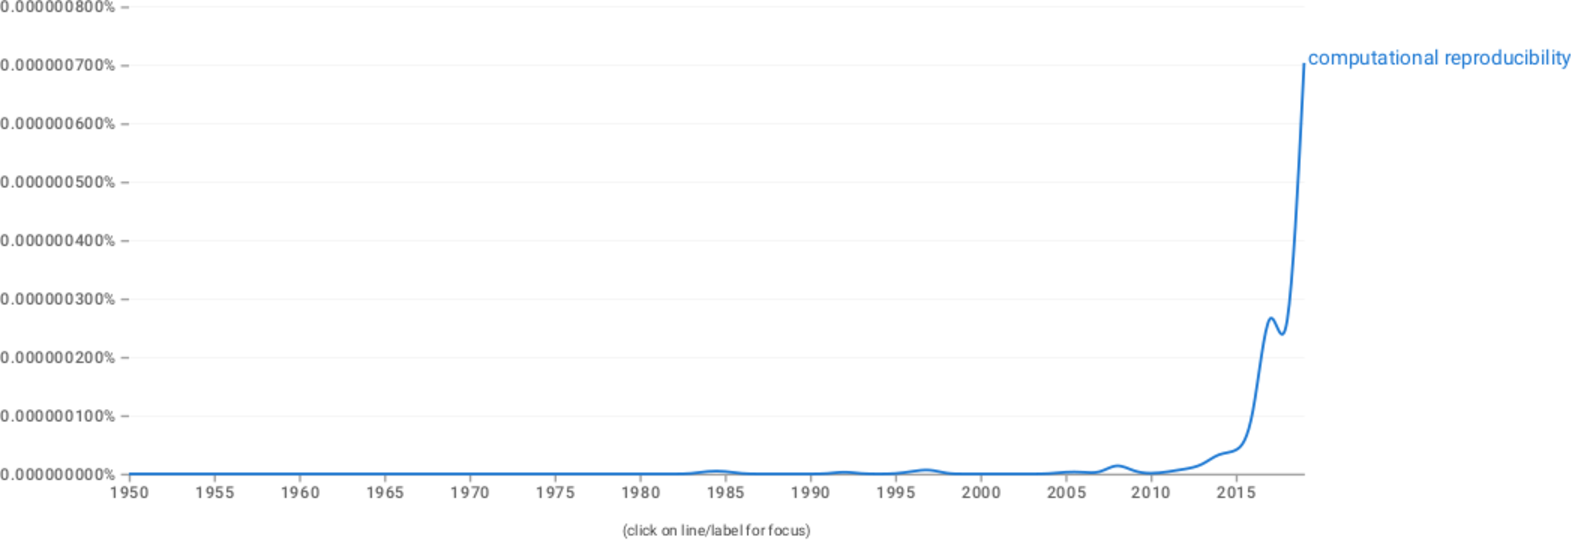
\includegraphics[width=\textwidth]{google_ngram_reproducibility_2023-05-08.pdf}
	\caption[Computational reproducibility in the literature]{Popularity of computational reproducibility: A chart of the frequencies of the n-gram ``computational reproducibility" (using yearly count, normalized be the numbers of publications in each year) in literature included in the English(2019) corpus of Google books. This graph has been created using the Google Ngram Viewer (\href{https://books.google.com/ngrams/info}{books.google.com/ngrams}) \citep{michel2011quantitative}}
	\label{fig:ngram}
\end{figure}


\subsection{``Everything matters'' for computational reproducibility in neuroimaging}

% maybe NARPS paper?`

As this definition of computational reproducibility implies, the building blocks of research output extend to more than the files that constitute the actual research output, but also to all elements involved in its generation \citep{claerbout1992electronic}.
Consider different types of research output:
Raw data originates from acquisitions based on - potentially ongoing - experiments, raw data transformations, or data cleaning.
Processed data or results stem from computations with analysis code or software in specific versions on particular data.
And software, expressed in raw (code) or derived (transformed into executable) form, is created or used in specific computational environments, with compilers, underlying libraries, and systems in distinct versions.
Consequently, these building blocks play an integral part in the genesis of research outputs, and changes in these building blocks or their composition can translate to changes in the resulting research output.\\
Because of their complexity, neuroimaging studies face obstacles for reproducibility.
For one, the details of how code, software, or data have been used to generate a research output, such as analysis parameterization, the subset of data used as input, or sequence and invocation of employed software tools, are volatile.
Shared code and data does not always suffice to reproduce a result:
A study of data availability, reusability, and reproducibility demonstrated that well-described, ``in principle reusable'' data often does not suffice to reproduce the scientific findings of the corresponding publications due to  missing process provenance metadata \citep{hardwicke2018data}.
Secondly, even if methods and their sequence are well-described, precise information about the employed software tools is crucial, too.
The fact that different neuroimaging analysis software can produce distinct results from the same data despite using similar conceptual methodology is well known \citep{bowring2019exploring}.
This has been attributed to implementation differences \citep{palumbo2019evaluation}, software errors \citep{eklund2016cluster}, or analytic configurations \citep{pauli2016exploring}.
For example, in task-based fMRI, \citet{li2021moving} found that the choice of output space or resolution can have a marked impact on variability between conceptually similar processing pipelines.
Moreover, even with identical pipelines and data, surprising result variability can occur with minor variations in parametrization.
\citet{mueller2017commentary} reported that the choice of resampling resolution impacts alpha inflation, and \citet{li2021moving} identified the decision whether or not to include global signal regression as a major source of intra-pipeline variation.
Finally, even the same analysis, with identical parametrization, software tool, and data, can result in different outcomes if it is repeated across different operating systems, or with differences in versions of a singular software tool or operating system \citep{gronenschild2012effects, glatard2015reproducibility}.
%more here
Computational reproducibility across computing environments thus often remains elusive unless accounted for from the very start.
Therefore, in addition to ``Everything matters'',  \citet{kennedy2019everything} cued the phrase ``Reproducible by Design (as opposed to reproducibility as an afterthought)'' for conducting research in a way that makes computational reproducibility possible.
The next section highlights a number of strategies for this.

% However, a growing number of studies suggest that differences in the implementation of these processing steps or how they are “glued together” can yield notably different outcomes. Studies systematically comparing specific preprocessing steps such as segmentation15, motion correction16, and registration17–19 have reported substantial variation in outputs generated across independently developed packages when applied to the same data. In the analysis of task fMRI data, end-to-end pipelines built using different software packages have been found to produce marked variation in the final results20–23. from https://www.biorxiv.org/content/10.1101/2021.12.01.470790v2.full


\section{Towards re-usable research objects}


The reusability of research objects has become a distinct characteristic of scientific practice as it allows for reproduction, verification, building up upon and extending existing work, evidence synthesis, and minimizing duplicate efforts in the advancement of science \citep{thanos2017research}.
With this, it maximizes the impact of the funding and work that resulted in the research output.
Its central role in the \gls{FAIR} principles \citep{wilkinson2016fair} and a variety of funding sources such as the Economic and Social Research Council (ESRC, UK), the European Research Council (ERC, EU), or the National Institutes of Health (NIH, US) are a testament to this.
In the scope of the FAIR principles, reusability focuses on the ability of a human or a machine to decide if data are useful and usable in a particular context.
This reusability requires trust \citep{bechhofer2013linked}: Re-users must be able to audit the steps performed in an experiment or analysis in order to be convinced of the validity of the results or derivatives.
FAIR principle R1.2, ``(Meta)data are associated with detailed provenance'' \citep{wilkinson2016fair}, refers to this.
This principle also encodes the process provenance necessary for reproducibility.
And indeed, reproducibility and trust are closely related:
Where resources are not fully FAIR yet, manual reproducibility typically yields the trust that process provenance would otherwise provide.
A new project, for example, commonly starts with a check if the previous foundational findings still hold.\\
As the FAIR principles advocate for richly curated metadata, many scientific fields or projects argue in favor of coordinated use of ontologies for metadata and brought forward efforts for ontology development and consensus building \citep[e.g.,][]{wise2019implementation, abrams2022standards, papadiamantis2020metadata}.
But not in all domains are the necessary metadata standards incentivized or ready to use.
A few years before the publication of the FAIR principles, \citet{bechhofer2010research} cued the term ``reusable research object'' in a conceptual position paper.
They describe it as a precursor of a FAIR research object, specifically as a ``container for a principled aggregation of resources, produced and consumed by common services and shareable within and across organisational boundaries [...that] includes not only the data used, and methods employed to produce and analyse that data, but also the people involved in the investigation. An association with a dataset (or service, or result collection, or instrument) is now more than just a citation or reference to that dataset (or service or result collection). The association is rather a link to that dataset (or service or result collection) that can be explicitly followed or dereferenced providing access to the actual resource and thus enactment of the service, query or retrieval of data, and so on.'' \citep{bechhofer2010research}.
This description matches characteristics that DataLad datasets or its contents can posses.
% Detail how datalad adheres to these requirements.
In the following, I will highlight four properties of research objects that can arise from pragmatic research data management -- versioned, actionable, modular, and portable -- and how these properties make them reusable  even if full FAIRness can not yet be achieved \citep{wagnerohbm2021}.
% and argue why the \gls{rdm} features that DataLad provides assist with FAIRification.

\subsubsection{Exhaustive versioning}

The information ``I generated X from data Y with software Z'' is insufficient for reproducibility and trustworthiness if Y exists in multiple versions or subsets, if different releases of Z have relevant implementation differences, or if Z behaves differently depending on the environment it is used in.
If digital research objects are exhaustively tracked, they can be accessed and used transparently in a uniquely identified version state.
This exhaustive identity registration removes ambiguity that arises if the files in question are not completely static.
Therefore, the first relevant feature that DataLad provides for reproducibility and reusability is version control for all relevant files -- from data to code to software environments.
In addition, this makes the DataLad dataset a suitable overlay structure to encompass every relevant element for a scientific project, laying the foundation to include all digital data, methods, and provenance as a reusable research object as \citet{bechhofer2010research} propose.
% make point about **exhaustive** tracking stronger

\subsubsection{Actionable metadata}

Process provenance metadata how a file came to be is often incomplete and difficult to retrace \citep{hardwicke2018data}.
As it is tedious, often without an immediate benefit for curators, and rarely explicitly incentivized to retrospectively annotate research objects with process provenance \citep{edwards2011science, san2009long}, this information should be captured at the time of creation, with the tools and persons that are involved in the creation of research outputs anyway \citep{dallas2016digital}.
But while early curation can increase the comprehensiveness of metadata, additional measures should guarantee its validity, as even fully described research outputs fail to be reproducible or reusable if their description or provenance contains errors \citep[see, e.g.,][]{manninen2017reproducibility}.
The most pragmatic approach to validate metadata is to base subsequent processing on them.
For a simple example, consider a codified parametrization of an analysis in a configuration or analysis design file  \citep[see, e.g.,][]{jas2018reproducible}:
If an analysis based on it completes successfully, it constitutes valid provenance metadata, created by an expert or automatically at the earliest possible time at no additional cost, and adds immediate benefit for curators as it captures relevant provenance and detects erroneous or missing metadata in passing.
Creation and validation is easiest if it is an automatic process within the research process, and if the tools used during the creation also use the same metadata that gets eventually published alongside the final research output.
Therefore, the actionable metadata DataLad can acquire from command executions are the second relevant property for reusability.
Even if this metadata does not follow established community standards as required by the \gls{FAIR} principles yet, it preserves knowledge that would otherwise be lost, without requiring additional training, impeding later additions, or putting additional burden on scientists - it is a byproduct of standard scientific practice.
The fact that it can be re-executed automatically, and that resulting recomputations are automatically compared to previous versions by employed version control tools, provides an effortless form of validation.


\subsubsection{Modular structure}

The reusability of scientific work can improve if it is accessible in modular units that constitute unambiguous multi-use components, such as raw data, processed data, or software.
In the simplest case, modularization means placing conceptually distinct content into separate files, and grouping files in individual directories to reflect more global structures.
Distinct units, such as the directories ``code/'' and ``inputs/'', increase transparency if each location is associated with distinguishable content, ease flexible recombination of such components into new projects, allow continuous evolution of an individual module without impact on other components of a project, and enable location-specific access control.
Though a single modular unit can not entail all relevant elements of a scientific study or data analysis, exhaustive tracking of all elements without sacrificing modularity can be achieved by linking multiple modular units in dependency relationships.
A useful metaphor are package management systems such as conda (\url{https://docs.conda.io}) or APT (\url{https://wiki.debian.org/Apt}): A software package is a modular unit, installed with a package manager.
However, packages usually depend on other software packages, which are listed as its ``dependencies''.
During installation, package managers check if all of the linked dependencies exist on the system, and if not, install them in the required versions automatically.
Thus, a third feature for reusability is modularity as provided with DataLad's subdataset mechanism.
In scientific projects, modular units (data, software, code) are the dependencies of a given research output.
When those units are tracked as datasets, dependency relationships in the form of subdatasets form actionable links with precise versions.
This mirrors the linked dependencies that \citet{bechhofer2010research} proposed.


\subsubsection{Portability}

The fourth property is portability.
The more portable a digital research object is, the easier it is to reuse it.
A research object is fully portable if no adjustments are necessary for it to function the way it is intended to on different computational infrastructure -- ideally even when used by a naive re-user with a different area of expertise (i.e., without domain knowledge).
The more adjustment or domain knowledge is necessary, the less portable a research output becomes.
A factor contributing to portability self-containment such that research outputs can be used or reproduced on different computational infrastructure by other users.
Completeness is crucial for this, and a research output should be accompanied by the necessary code, data, and computational environment to produce it.
Self-containment also entails that a project can be moved across computers and remains functional without adjustment, for example by ensuring that no references to file system, operating system, or user specific idiosyncrasies are included.
Only if a re-user does not need to modify project files, they can be certain that they did not inadvertently break or influence the output with it.

\begin{figure}
	\centering
	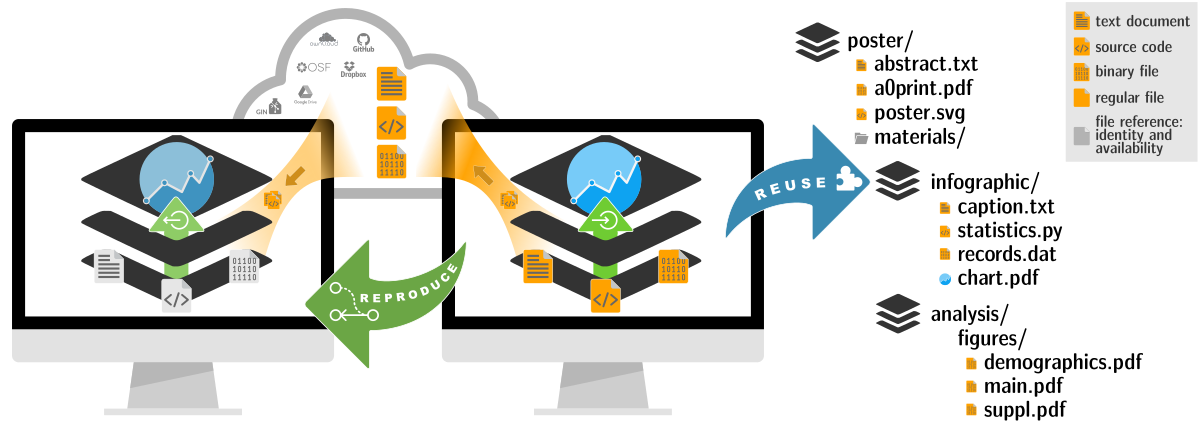
\includegraphics[width=.9\textwidth]{vamp.png}
	\caption[DataLad datasets as reusable research objects]{Reusing research outputs implies trust, and trust should be earned through verification. Verification is enabled by provenance information. Provenance capture of research outcomes requires exhaustive tracking of all inputs, as well as process records that describe how inputs were combined and transformed to generate outputs (middle). When lightweight metadata are actionable, they can be used to reproduce research outputs in a different environment from precisely identified inputs by (re-)applying the recorded process (left). A data structure that affords this type of portable recomputation is a self-contained unit that can be reused as a modular input component for incremental research (right).
	}
	\label{fig:vamp}
\end{figure}




% curation needs to be pragmatic

Although FAIR research objects are universally desirable, in practice, the necessary standards and procedures for creating FAIR (meta)data are not always already in place when research is conducted.
This can turn FAIRification into a bureaucratic data governance effort, diminishing the immediately obvious benefits for the curator \citep{zehl2016handling}.
However, the four properties outlined above are a big step into the right direction, and essentially a byproduct from pragmatic research data management in DataLad datasets.
\cref{fig:vamp} illustrates how it yields trusted and reusable research objects, and the next section details a technical implementation and proof-of-concept analysis to create such reusable research objects as a byproduct of \gls{rdm} in analyses of any scale.

\pagebreak

\section{FAIRly big: A framework for computationally reproducible processing of large-scale data}

The following section is a short overview of our original publication \citet{wagner2022fairly}. The reader is invited to visit the published paper for further details.

Large-scale datasets pose additional challenges for \gls{FAIR} research objects.
Their storage and computational demands increasingly exceed common \gls{HPC} infrastructure, and computing procedures that are common in fields accustomed to smaller datasets such as storing multiple copies of the data become infeasible \citep{horien2021hitchhiker}.
As the complexity of reproducing and verifying large scale datasets growths, the trustworthiness of derivative data decreases.
And as data processing results often multiply storage demands, keeping intermediate outcomes on disk is rendered increasingly prohibitive, which further impedes the possibility to retrace the origin of research outcomes.
Yet for large scale datasets specifically, sharing data derivatives is the most -- or sometimes the only -- viable way to extend previous research \citep{craddock2013neuro}:
It opens up research opportunities to scholars without access to adequate computational resources, and minimizes duplicate analysis efforts for resource-heavy, costly computations with considerable environmental impact \citep{portegies2020ecological}.\\
Based on DataLad, containerization software, and job scheduling systems, we build a portable, free and open source framework to reproducibly process large-scale datasets.
It applies workflows from software engineering -- in particular distributed development -- to computational research, and empowers reusers to automatically reproduce results based on machine-actionable records of computational provenance without access to the original infrastructure.
For this, it puts the aforementioned properties in practice, using DataLad datasets as a comprehensive data structure to track all elements of digital processing, perform portable computing in automatically bootstrapped ephemeral workspaces, and capture validated and re-executable process provenance records.

\subsection{Framework overview}


\begin{figure}
	\centering
	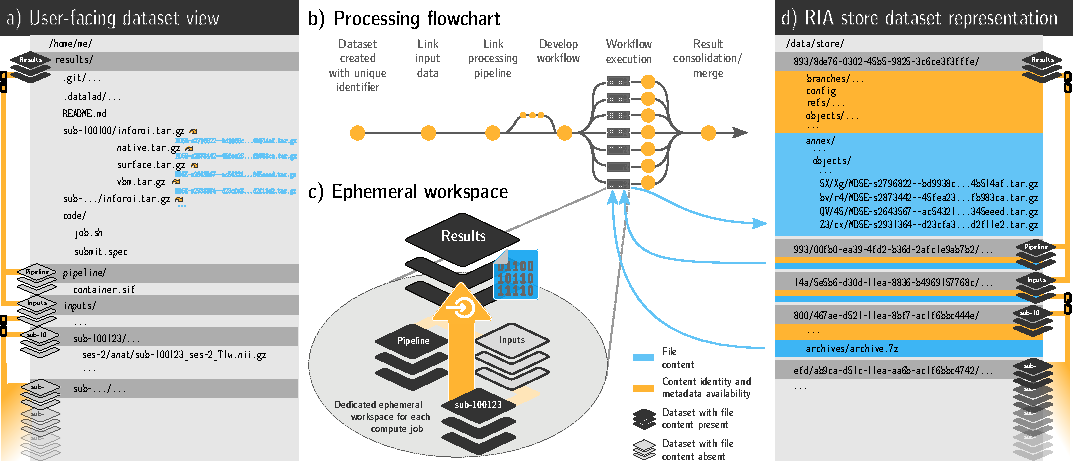
\includegraphics[width=\textwidth]{ukbworkflow_simplified.pdf}
	\caption[Schematic overview of the processing framework]{Schematic overview of the processing framework. a) The user-facing representation of the results on a file system after completed processing: A lean DataLad dataset that tracks the computed results, links input data and pipeline, and contains actionable process provenance and location information, allowing on-demand file retrieval or recomputation. Depicted files are from the UK Biobank showcase. b) Process-flowchart: First, a DataLad dataset links required processing components (e.g., input data, processing pipeline, additional scripts). Next, compute jobs are executed, if possible in parallel. Afterwards, results and provenance are aggregated (merged). c) An ephemeral (short-lived) compute workspace: Each compute job creates a temporary, lean clone, which retrieves only relevant subsets of data, and captures the processing execution as provenance. After completion, results and provenance are pushed into permanent storage (see d), and the ephemeral workspace is purged. d) The internal dataset representation in a RIA store: The store receives results and can contain input data, optionally using compressed archives (for reduced disk space/inode consumption) or encryption during storage and transport. It is the only place where results take up permanent disk space. If inputs are available from other infrastructure (external, web-accessible servers, cloud infrastructure), jobs can obtain them from registered sources, removing the need for duplicate storage of input data.}
	\label{fig:fairly_workflow}
\end{figure}


The framework combines distributed version control systems, containerization software, job scheduling tools, and storage solutions with optional encryption and compression into a sequential analysis workflow (\cref{fig:fairly_workflow}).
Its setup is as follows:\\
The start and end point of the workflow is a portable DataLad dataset that contains the exact identity and location of all data processing inputs and, eventually, the re-executable processing results (\cref{fig:fairly_workflow}a).
In a first step, it is assembled from all relevant processing components, most commonly input data and software containers with computational environments or pipelines.
The use of software containers, while not strictly required, is a practical method to provide portable computational environments and forgo a number of challenges that computational reproducibility otherwise poses.
To harvest the advantages of modularity, processing components are placed in separate DataLad datasets and linked as subdatasets.
To provide features that are necessary for processing personal large-scale data, such as encryption (to comply with data protection regulations), compression (to save disk space), and composition to archive files (to reduce the number of files),
DataLad datasets involved in the workflow are placed into so-called RIA stores \citep{poldrackRIA}.
This ``backend'' representation stores a dataset of any size in 25 files, with optional compression and encryption.
\cref{fig:fairly_workflow}a illustrates a DataLad dataset's front-end structure when cloned in a user's workspace, and \cref{fig:fairly_workflow}d shows its RIA representation.\\
Based on this self-contained structure, the framework needs to conduct user-defined processing in a way that captures and validates actionable metadata.
While DataLad's \texttt{containers-run} functionality supports the capture, simultaneous validation requires additional tweaks.
For this, the framework bootstraps an entire temporary analysis environment from scratch based on the information contained in the initial dataset (\cref{fig:fairly_workflow}c).
In this ephemeral environment, processing is solely based on information already recorded in the dataset.
As the computation is invoked with a provenance capturing \texttt{datalad containers-run} command, results and provenance are saved automatically if the analysis succeeds.
And this success is evidence that existing information is valid and sufficient to make the dataset portable.\\
The basis for these ephemeral workspaces is the ability to distribute DataLad datasets across local or remote infrastructure as lightweight, linked clones, and the process mirrors a software development routine, where changes are developed in a distributed network:
An orchestration layer clones the DataLad dataset into a temporary location, uses its recorded history to infer relevant details about precessing components, and add results on top of it.
Afterwards, results and their provenance can be pushed back before the ephemeral workspace is purged.
To ensure that this orchestration can scale, it needs to support parallel executions, i.e., several analyses running in ephemeral workspaces at the same time.
This is complicated in Git repositories as concurrent processes can interfere with one another.
Two techniques, again adopted from distributed software development, make it possible.
The first consists of duplicating the DataLad dataset that is used as an analysis starting point into two clones: One remains unaltered and acts as an input source from which the ephemeral clones are bootstrapped (\cref{fig:fairly_workflow}a).
The other one acts as the target location for results.
This separation prevents concurrent clone and push operations without duplicating file storage.
The second technique involves the use of branches, independent segments of a DataLad dataset's history that allow for parallel developments based on a common starting point.
Each individual ephemeral workspace saves its results and provenance on a unique branch.
When several parallel ephemeral clones push their individual histories into a single location, they thus do not conflict with one another.
This process mirrors feature development in software projects where a mainline branch contains agreed upon code.
Changes are build on top of the mainline code, but in branches such that concurrent developments of several contributors do not conflict, and later, a so-called \texttt{merge} can integrate a branch into another one.
The clone and push orchestration is implemented as a job script that wraps the execution of the analysis.
\cref{lst:job} contains an example bash script:
The clone source and push target locations are provided as parameters to the script (lines 5-6).
Then, the dataset is cloned from the specified source (line 11), the dataset for results is registered (line 17), and a unique branch is created (line 21).
Afterwards, analysis-specific code can run, and as a last step, its results and provenance are pushed into the destination dataset (lines 44, 49).\\
Running such a script performs one computation in one ephemeral workspace.
If one breaks the analysis into parts, for example one preprocessing pipeline per participant in a dataset, a job scheduling system can assist in deploying thousands of computations in parallel.
For this, the framework supports to major job schedulers, HTCondor and SLURM, natively.


Finally, once the results from all ephemeral workspaces are aggregated in branches in the target dataset, they are merged into the mainline branch using a Git octopus merge.
With the exception of merging all results, the entire setup can be bootstrapped automatically with an openly shared shell script.





\begin{Listing}
	\centering
	\lstset{
		language=bash,
		basicstyle=\ttfamily\footnotesize,
		breakatwhitespace=true,
		breaklines=true,
		breakindent=-0pt,
		postbreak=\raisebox{0ex}[0ex][0ex]{\ensuremath{\hookrightarrow\space}},
		captionpos=b,
		commentstyle=\color{dataladblue!60!black},
		firstnumber=1,
		keepspaces=true,                 % keeps spaces in text, useful for keeping indentation of code (possibly needs columns=flexible)
		%keywordstyle=\color{blue!70!black},
		numbers=left,                    % where to put the line-numbers; possible values are (none, left, right)
		numbersep=3pt,                   % how far the line-numbers are from the code
		numberstyle=\tiny\color{gray}, % the style that is used for the line-numbers
		rulecolor=\color{black},         % if not set, the frame-color may be changed on line-breaks within not-black text (e.g. comments (green here))
		showspaces=false,                % show spaces everywhere adding particular underscores; it overrides 'showstringspaces'
		showstringspaces=false,          % underline spaces within strings only
		showtabs=false,                  % show tabs within strings adding particular underscores
		stepnumber=1,                    % the step between two line-numbers. If it's 1, each line will be numbered
		stringstyle=\color{dataladyellow!70!black},     % string literal style
		tabsize=2,
		xleftmargin=1em,
	}
	% our separation of input and output store still bothers me, this could have
	% been avoided with a bit more thinking, but oh well, too late now
	\begin{lstlisting}[multicols=2]
		#!/bin/bash
		# fail on any issue, show commands
		set -e -u -x
		# name arguments for readability
		dssource="$1"
		pushgitremote="$2"
		subid="$3"

		# obtain the analysis dataset, which
		# also tracks the required inputs
		datalad clone "${dssource}" ds
		cd ds

		# register location for result
		# deposition, separate from the input
		# source for performance reasons only
		git remote add outputstore "$pushgitremote"

		# all job results will be put into
		# a job-specific, dedicated branch
		git checkout -b "job-$JOBID"

		# START OF APPLICATION-SPECIFIC CODE
		# pull down input data manually,
		# only needed for wildcard-based file
		# selection in the next command
		datalad get -n "inputs/ukb/${subid}"
		# datalad containers-run executes
		# the "cat" computational pipeline.
		# specified inputs are auto-obtained,
		# specified outputs are saved with
		# provenance record
		datalad containers-run \
		-m "Compute subject ${subid}" \
		-n cat \
		--explicit \
		--output "${subid}" \
		--input "inputs/ukb/${subid}/*T1w.nii.gz"
		"<container invokation arguments>"
		# END OF APPLICATION-SPECIFIC CODE

		# push result file content to the
		# configured "storage-remote"
		datalad push --to storage-remote

		# push branch with provenance records
		# needs a global lock to prevent
		# write conflicts
		flock "$DSLOCKFILE" git push outputstore

		# log entry to mark non-error exit
		echo SUCCESS
	\end{lstlisting}

	% max 250, is 190
	\caption[Job orchestration for parallel processing]{Complete compute job implementation as a bash script.
		A batch system invokes the job-script in a temporary working directory with three parameters:
		a URL of a DataLad dataset tracking all code and input data,
		a URL to deposit job-results at, and
		an identifier to select a sample for processing.
		%
		Apart from performance-related optimizations, the job implementation conducts three main steps:
		1)~\texttt{clone} a DataLad dataset with all information to bootstrap an ephemeral computing environment for each job;
		2)~\texttt{containers-run} a containerized pipeline with a comprehensive specification of to-be-retrieved inputs and to-be-captured outputs;
		3)~\texttt{push} captured outputs and process provenance records to a permanent storage location.
		%
		Preparation, computation, provenance record creation, and file content deposition on permanent storage are fully independent across jobs, and are executed in parallel.
		Only the \texttt{git push} of the provenance record to a central repository must be protected against concurrent write-access for technical reasons.
		Additional job parametrization (\texttt{DSLOCKFILE} and \texttt{JOBID} environment variables) are defined at job-submission using batch system specific means.
		The job script can be adjusted to a different processing pipeline by replacing the container invocation (see \texttt{APPLICATION-SPECIFIC CODE} markers).}
	\label{lst:job}
\end{Listing}


\subsection{Proof-of-concept analysis}

In a proof-of-concept analysis, we applied the framework to run a containerized pipeline for \gls{vbm} \citep{ashburner2000voxel} from the \gls{CAT} \citep{gaser} on data from the UKB project \citep[][comprising 76 TB in 43 million files under strict usage constraints]{matthews2015uk}.
An overview of the analyis is shown in \cref{fig:fairly_datasets}, and the setup steps are publicly available as a bootstrap script\footnote{\url{https://github.com/psychoinformatics-de/fairly-big-processing-workflow/blob/main/bootstrap_ukb_cat.sh}}.

\begin{figure}
	\centering
	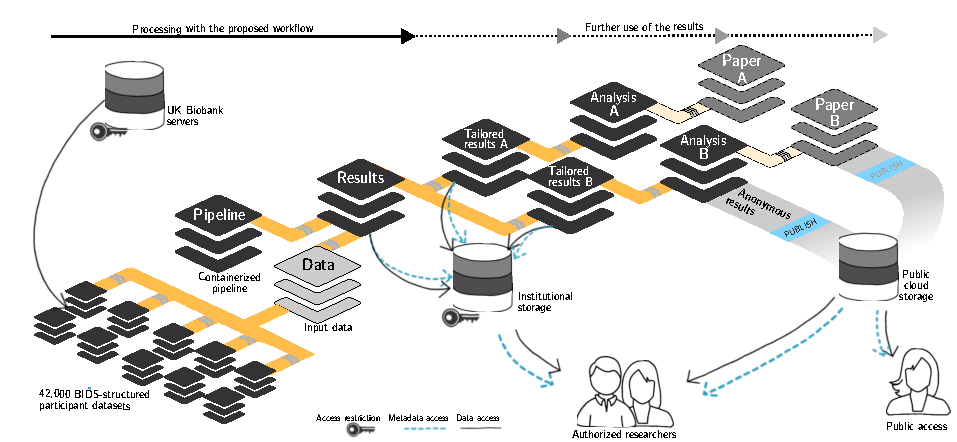
\includegraphics[width=\textwidth]{ukb_datasets.pdf}
	\caption[Overview of DataLad dataset linkage through processing and reuse]{Any DataLad dataset may comprise other DataLad datasets as subdatasets via lightweight but actionable and versioned links. This connects a dataset to the content and provenance of a different modular unit of data, such as the outcomes of a the preceding processing step. The genesis of an analysis output (Analysis A/B) based on intermediate processing outcomes (Tailored results A/B) can thus be traced back all the way to the original raw data. Access control and storage choices are independent across individual components in this network of linked data modules. Aggregated data and analysis results can be shared with larger audiences or publicly on a variety of platforms, while raw and derived data may underlie particular access restrictions, or require particular hosting solutions due to their size.}
	\label{fig:fairly_datasets}
\end{figure}

\subsubsection{Workflow setup}

First, using the DataLad extension \texttt{datalad-ukbiobank} \citep{hanke_michael_2022_7296550}, we retrieved MRI data into one DataLad dataset per participant and restructured it to BIDS \citep{gorgolewski2016brain}, yielding 42,715 datasets in total.
A single superdataset (``Data'' in \cref{fig:fairly_datasets}) tracks them using about 40 MB of space.
It is installable within seconds to retrieve any registered file content in the DataLad dataset hierarchy on demand.\\
To set up a processing pipeline, we built a Singularity container for the Computational Anatomy Toolbox \citep[CAT; version: CAT12.7-RC2, r1720]{gaser}, which is an extension to the Statistical Parametric Mapping software (SPM; version: SPM12, r7771; \url{www.fil.ion.ucl.ac.uk/spm/software})\footnote{A detailed description and full recipe of the container together with instructions on how to build and use it is publicly available at \url{github.com/m-wierzba/cat-container}.}.
From it, we chose \gls{CAT}'s default segmentation of structural T1-weighted images using geodesic shooting \citep{ashburner2011diffeomorphic}, including calculation of total \gls{GM}, \gls{WM}, and \gls{TIV}, as well as extraction of regional \gls{GM} estimates from several brain parcellations.
We then linked these two inputs as subdatasets to the processing dataset (``Results'' in \cref{fig:fairly_datasets}), and added two custom code files.
First, a batch script with \gls{CAT}'s processing steps and parameterization, which bundled up all relevant analysis steps into single command.
This script runs per image, and constitutes the smallest unit for recomputation.
And second, a utility script to post-process all relevant outputs with a focus to reduce the number of files and artificial variations between recomputations.
For this, it stripped results of timestamps and other non-deterministic log file content, and used the \texttt{tar} utility to bundle \gls{vbm} results into four reproducibly organized archives according to envisioned consumption scenarios (see \cref{fig:fairly_workflow}a).
These measures were taken to obtain a meaningful estimate of intra-pipeline variability across recomputations, and to keep the number of files in the resulting dataset in a manageable range.\\
%After all required processing elements were either included or linked, we stored all DataLad datasets in a RIA store:
%A single participant dataset with several hundreds of files is represented in 25 inodes and about 4 GB of disk space in a RIA store, and in total, the employed RIA store hosts 42,715 datasets comprising the full UKB data with less than 940k inodes.\\
To test the frameworks portability and estimate result variability across computations, we set the analysis up to run on two systems, a \gls{HPC} cluster and a \gls{HTC} cluster.
Each system imposed different resource constraints.
The \gls{HPC} system, a modular supercomputer with abundant disk space and compute power \citep{krause2018jureca}, imposed an inode quota, a limit on the total number of files, of 4.4 million – less than the total number of files of the raw dataset.
The \gls{HTC} cluster, in contrast, was constrained on storage capacity, preventing the existence of more than one copy of the raw dataset, and limiting the size of derivatives that could be stored.
The workflow was thus setup identically across the employed systems apart from the implementation of job submission, which accounted for platform specific idiosyncrasies such as these restrictions.
Irrespective of system, one compute job per participant was generated.
This compute job serially processed all available anatomical images for a given participant.
For each image, a dedicated provenance record was captured, yielding a total of 41,180 records.
The platform-specific job submission scripts were implemented for SLURM and HTCondor, respectively.
We adjusted the job load to the available disk space or inode resources when disk space or inode availability were insufficient for the full dataset by scheduling only as many jobs in parallel as there were resources to handle extracted inputs.

\subsubsection{Workflow execution and consolidation}

On the \gls{HPC} system we completed data processing for the one-hour-per-image pipeline within 10.5 hours, using 25 dedicated compute nodes, each executing 125 jobs in parallel on RAM disks with GNU Parallel \citep{tange2011gnu}.
On the \gls{HTC} system in turn, computations were scheduled dynamically across several weeks.
On both systems, recorded outputs and provenance records amounted to a total of 995.6 GB of computed derivatives in 163,212 files.
After completion, result were consolidated by merging result branches, yielding a collection of different VBM-related measures for all images in the sample, represented in archives, and annotated with re-executable provenance records in a DataLad dataset.\\
This DataLad dataset was subsampled into smaller ``special purpose'' datasets tuned for specific research questions, containing extracted and optionally aggregated subsets of the results for easier consumption and faster access.
For this, the main result DataLad dataset became an input to a new tailored DataLad dataset via nesting (``Tailored results A/B'' in \cref{fig:fairly_workflow}), which extracted and transformed required files with provenance tracking by \texttt{datalad run}.
If underlying large-scale computation is redone or extended, the subsampled datasets can be updated by re-applying this transformation via \texttt{datalad rerun}.
And throughout the dataset hierarchy -- using the encoded, machine-actionable provenance information -- a single result can be traced to the precise files they were generated from in a transparent and reproducible manner.
The direct computational output of the proof-of-concept framework execution is therefore not a final result, but an intermediate representation optimized for storage and handling.
As more tailored views for concrete use cases can be flexibly and reproducibly created, we achieve a compromise between the desires of a data consumer and the demands of the storage infrastructure and operators for such large scale datasets.

\subsubsection{Intra-pipeline variability}

In order to investigate intra-pipeline variability, the result consolidation described above was first performed separately on each computational infrastructure.
Afterwards, the two complete sets of results were integrated in the same dataset, as two different branches, to estimate result variability.
With the exception of execution time, the number of jobs, proportion of successful jobs, and size and structure of the results were identical between the two systems\footnote{The difference in computational performance can be seen in a visualization of provenance information at \url{youtube.com/watch?v=UsW6xN2f2jc}. This visualization was awarded second place in the category videos \& animations in the 2021 \gls{ohbm} Brain Art Competition.}.
As content identity is precisely captured, bit-identical recomputations are easy to identify.
One type of the created output archives, surface and thickness projections, never yielded bit-identical results across computations.
But among the other three types of archives (modulated gray matter density and partial volume estimates in template space, atlas projections and partial volumes in individual space, and regional volume and thickness estimates of several atlases/parcellations), more than 50\% of all output files were bit-identical across the two computations.
A closer investigation of non-identical results revealed that outcome variability was largely attributable to minor numerical differences.
We illustrated the amount of dissimilarity by computing the \gls{mse} over recomputations for a range of key VBM estimates.
They can be found in \cref{tab:fairly_mse}.
We also correlated \gls{vbm} estimate distributions across recomputations for different brain parcellations included in the CAT toolbox output.
The lowest observed correlation were Pearson’s $\rho > 0.998$ for the Destrieux 2009 surface parcellation \citep{destrieux2010automatic} for all brain regions.
Finally, we derived quality control metrics for anatomical images from the computed results \citep{dahnke_retrospective_2013,dahnke_quality_2015} and correlated them across results.
They exhibit $\rho > 0.99999$ for computation and recomputation.


\begin{table}
	\centering
	\begin{tabular}{lcc}
		\toprule
		measure & $\mu$ & \gls{mse} \\ \midrule
		total surface area & 1891 & 0.315 \\
		cerebro-spinal fluid & 365 & 0.052 \\
        total intracranial volume & 1508 & 0.052\\
        white matter & 519 & 0.004\\
        gray matter & 621 & 0.001\\
		\bottomrule
	\end{tabular}
	\caption[Mean and mean squared error of results across computations]{Mean and mean squared error of results across computations}
	\label{tab:fairly_mse}
\end{table}


\subsubsection{Infrastructure-agnostic reproducibility}

%% rephrase!
To confirm the practicality of computational reproducibility solely based on the captured computational provenance information, we performed automatic recomputation of individual results on a consumer-grade, personal laptop without job scheduling.
%% rephrase!
This type of spot-checking results resembles the scenario of an interested reader or reviewer of a scientific publication with access to (parts of) the data, but no access to adequate large-scale computing resources.
%%rephrase
The recomputation solely relied on the local availability of the Singularity container technology, but was otherwise fully automatic.
Its success confirmed that platform idiosyncrasies were confined to the outer job scheduling layer only, and that the resulting research object was portable and across infrastructures.


\subsection{Future steps}


Building up on the framework, CITE-BABS has been created.


\begin{figure}
	\centering
	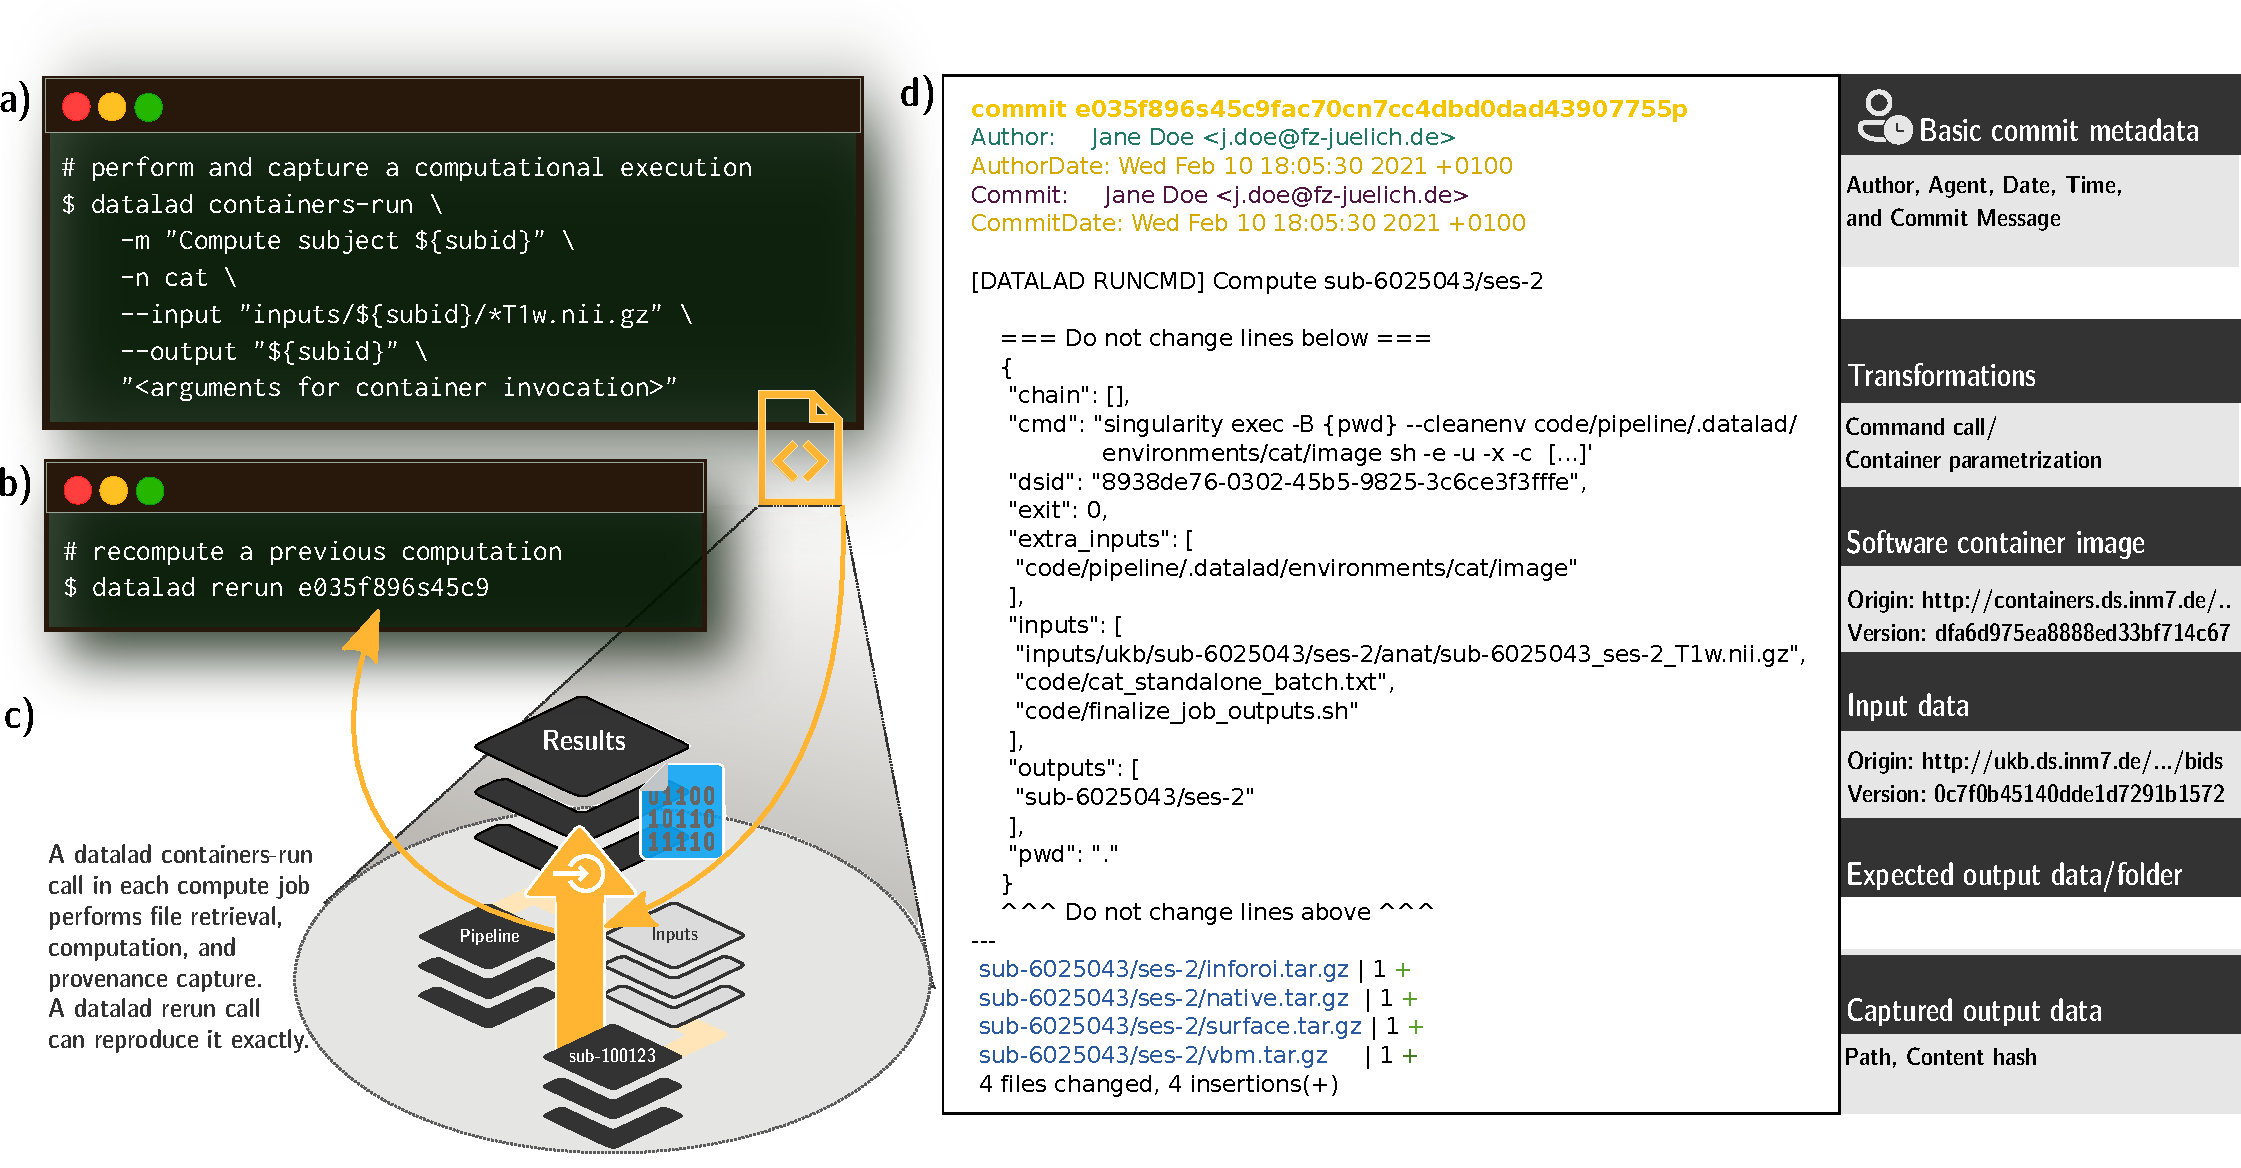
\includegraphics[width=\textwidth]{coarsemetadata.pdf}
	\caption[Process provenance of an individual job]{Process provenance of an individual job, its generation, and re-execution. a) Actionable process provenance is generated with a datalad containers-run command. This example contains a container name specification (cat), a container parametrization or command, a commit message, and an input and output data specification. The provenance is stored as a structured, JSON-formatted record linked to a Git commit. b) To re-execute a process, the datalad rerun command only needs to be parameterized with a revision identifier, such as a Git tag, a “commit shasum” (e035f896s45c9fa[...] in this example), or a revision range containing one or more commits with associated provenance records. c) The datalad containers-run call is at the center of each individual job. As the core execution command (see Listing 1, line 33-39), it performs data retrieval, container execution, and result capture, and generates the actionable provenance that a subsequent datalad rerun command (b) can re-execute. With complete provenance, a re-execution is supported on the original hardware, or on different infrastructure. d) The machine-readable, re-executable provenance record stored alongside computed results in the revision history. A legend (right) highlights the most important pieces of recorded provenance. While automatic re-execution requires the tool DataLad, sufficient information to repeat a computation using other means can also be inferred from the structured JSON records by other software or even humans. This information forms the basis for standardized provenance reporting, for example using the PROV data model 27.}
	\label{fig:fairly_metadata}
\end{figure}

% on re-analyzing the pipeline, cite li2021moving: "we demonstrated the role that pipeline replication can play as a means of exploring analytic variation and assessing the robustness of findings. To this end, we leveraged and extended the flexibility of C-PAC to replicate non-MATLAB dependent minimal processing pipelines (ABCD-BIDS, CCS, fMRIPrep-LTS) in a single platform"


\pagebreak


One way to track digital files is
While it is possible to exhaustively track all elements involved in a project with version control, industry use differs from RDM demands in science.
In industry contexts, it is primarily employed in software engineering for small-sized text files (source code). Science often works with large amounts of potentially sizable or binary files.
To exhaustively track all elements involved in a scientific project, large and binary files such as data and computational environments need to be versioned, too.
The concept of software containers - portable, light-weight software environments - make it possible to encapsulate computational environments as in-principle trackable elements, and a range of tools provide the ability to track even terabyte-sized and binary files.
Overall, version control is a well-established and reliable tool in industry and science. It can be employed at any point during a project, and yields a hands-on digital notebook of a project.
By extending its use beyond small-sized files to any digital research outputs and everything involved in its generation, version control can not only constitute established and beneficial research data management, but also lay the foundation for reusability by exhaustively tracking relevant digital elements and making them identifiable in precise versions.

From Donoho Buckheit 2015: Performance has everything to do with specifics: exactly what was done (which wavelets,
which coders, which detectors, which corpus of data) with exactly what parameters. In
this setting, publishing figures or results without the complete software environment could
be compared to a mathematician publishing an announcement of a mathematical theorem
without giving the proof. Waveleticians ought to publish their complete computational
environments


As highlighted in the Introduction, digital research outputs are the by- or end-products of scientific studies or analyses, from code, software, raw data or processed data, to analysis results or papers.
